% Roll Number 10, Alina Annie furtado
.
\textbf{\textcolor{LightMagenta}{Explain how SVM can be used for classification of linearly separable data. (May 2019, Qn 17(a)) \hfill (Mark 6)}} \\[5pt]
SVM, also known as Support vector machines can be used for both classification and
regression problems. But it is mostly used in classification problems. The objective of
the support vector machine algorithm is to find a hyperplane in an N-dimensional space
that distinctly classifies the data points. Consider the data points given below,
 \begin{figure}[htp]
    \centering
    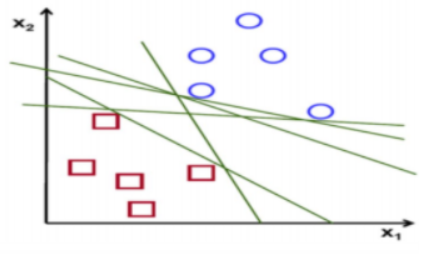
\includegraphics[width=5cm]{Images/A37_img1.png}
 \end{figure}
As you can see in the figure, the two data points can be separated in n number of ways
by using a straight line. But our aim is to find out an optimal hyperplane that efficiently
classifies the two data points. 
The main terminologies associated with  SVM are:\\
% \begin{enumerate}
%     \item Optimal Hyperplane
%     \item Marginal Planes
%     \item Marginal Distance
%     \item Support vectors
% \end{enumerate}
a) Optimal Hyperplane\\
b) Marginal Planes\\
c) Marginal Distance\\
d) Support vectors\\

Once the hyperplane is obtained, we obtain two planes that are parallel to the hyperplane and which pass through the data points which is nearest to the hyperplane.
 \begin{figure}[htp]
    \centering
    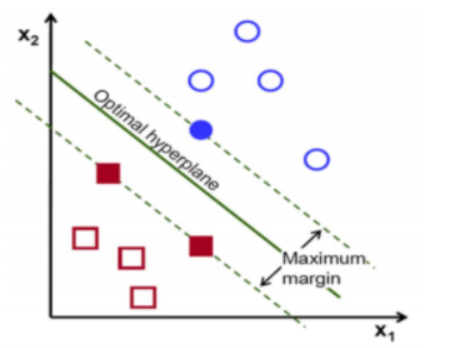
\includegraphics[width=5cm]{Images/A37_img2.png}
 \end{figure}
 Here in the second figure, we can see two parallel planes(Marginal planes) which pass connecting the data points which are nearest to the hyperplane. The distance between the two marginal planes is calculated by \(\frac{2}{{\vert}w{\vert}} \)
(where w is a unit vector) and is called Marginal distance.
 
 %{\lvert}2/w{\lvert} (where w is a unit vector) and is called Marginal distance.
 

 Support vectors are nothing but the nearest data points to the hyperplane. It can also be defined as the points which pass through the marginal plane. Our aim is to always obtain a generalised model. Therefore we must select the optimal hyperplane as the plane which is having the maximum marginal distance. The greater the marginal distance more will be the efficiency in classifying data points into the corresponding classes. This is how SVM can be used for the classification of linearly separable data.
